\documentclass[12pt]{article}


\usepackage{amssymb}
\usepackage{amsmath}
\usepackage{fullpage}
\usepackage{epsfig}
\usepackage{epstopdf}
\everymath{\displaystyle}
\usepackage{enumerate}

\newif\ifans

\ansfalse

\begin{document}

\begin{center}
\underline{\LARGE{Chapter 3.1: Angles \& The Unit Circle}}
\end{center}

\subsection*{Expected Skills:}

\begin{itemize}

\item Be able to sketch a standard position angle expressed in either degree or radian measurement.

\item Be able to convert between degree and radian measurement.

\item Be able to label points on the unit circle corresponding to angles of $30^\circ$, $45^\circ$, $60^\circ$, and related angles.

\item Be able to label points on the unit circle corresponding to the quadrantal angles.

\item Be able to find the length of a circular arc and the area of a sector of a circle.

\end{itemize}

\subsection*{Practice Problems: }

\begin{enumerate}

\item Label all of the indicated points on the unit circle, shown below.  Also, convert all of the angles from radian measurement to degree measurement.

\begin{center}
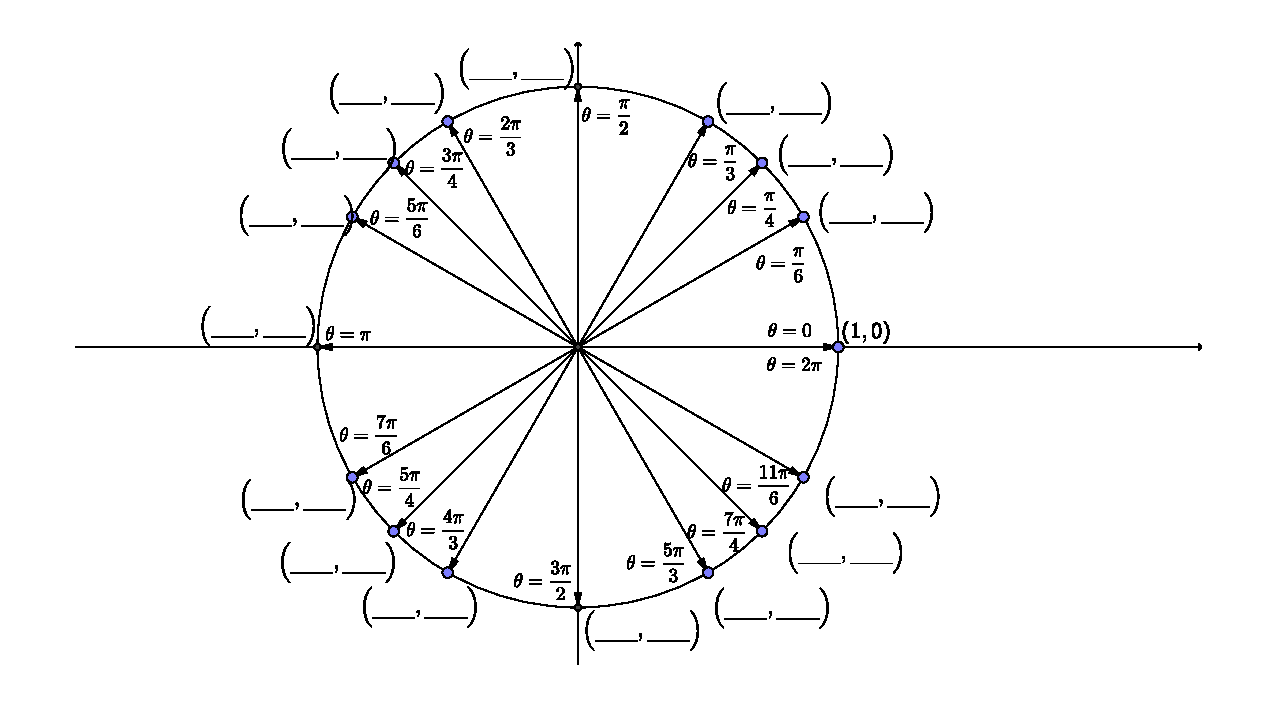
\includegraphics[scale=0.8]{unitcircle4.pdf}
\end{center}

\ifans{\fbox{\includegraphics[scale=0.5]{unit_circle.pdf}}} \fi

\newpage

\item Convert the following angles from degrees to radians.  Sketch each angle in standard position (i.e., with the initial side on the positive $x$-axis).

\begin{enumerate}

\item $\displaystyle 115^{\circ}$

\ifans \fbox{\parbox{1\linewidth}{$\displaystyle \frac{23\pi}{36}$; \\
\begin{center}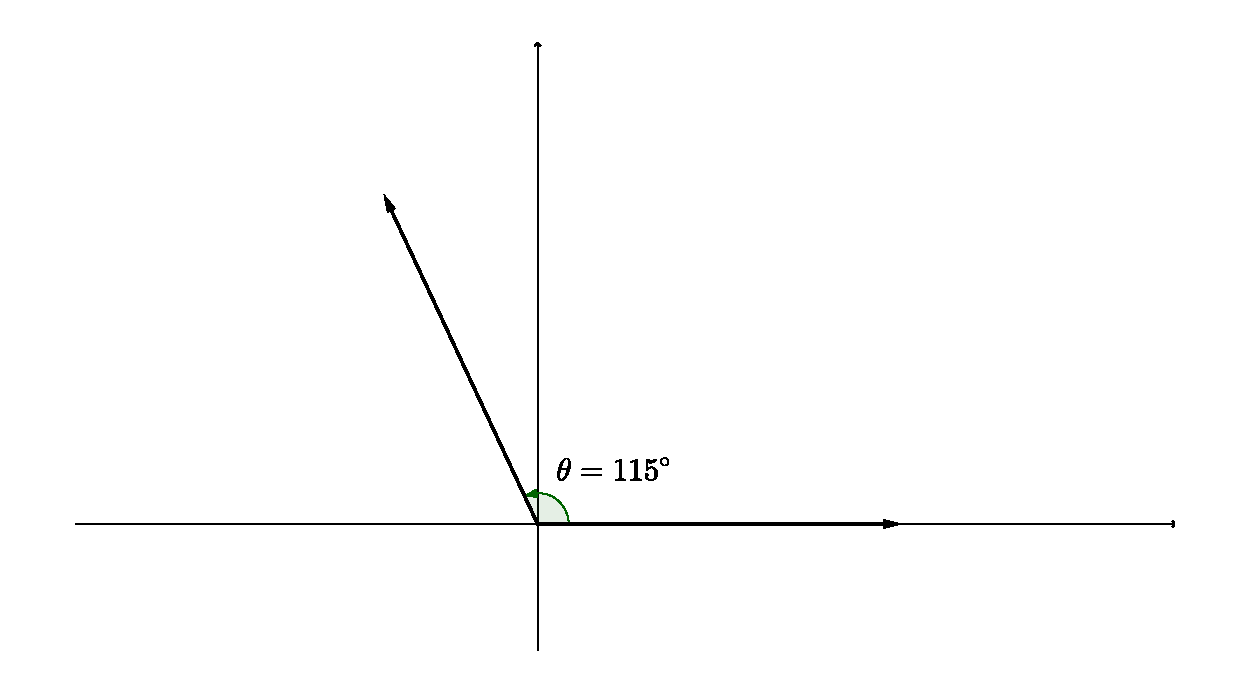
\includegraphics[scale=0.4]{115.pdf}
\end{center}}} \fi

\item $\displaystyle -150^{\circ}$

\ifans \fbox{\parbox{1\linewidth}{$\displaystyle -\frac{5\pi}{6}$;
\begin{center}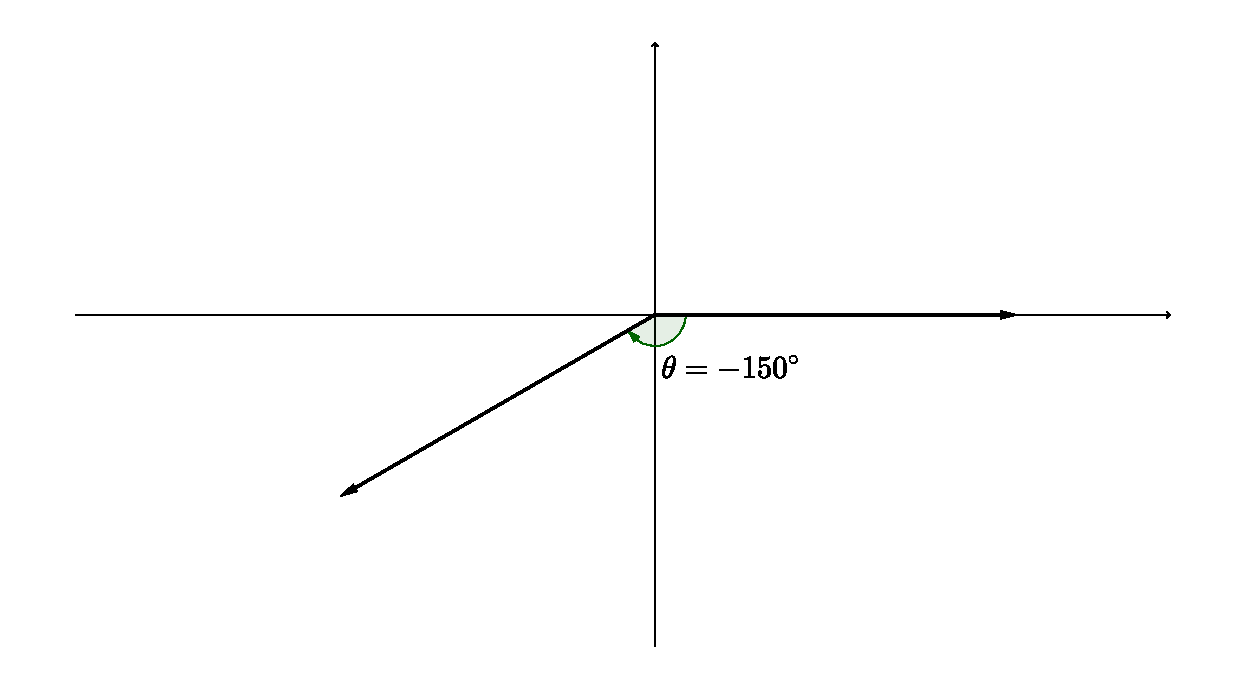
\includegraphics[scale=0.4]{-150.pdf}
\end{center}}} \fi

\item $\displaystyle 63^{\circ}$

\ifans \fbox{\parbox{1\linewidth}{$\displaystyle \frac{7\pi}{20}$; 
\begin{center}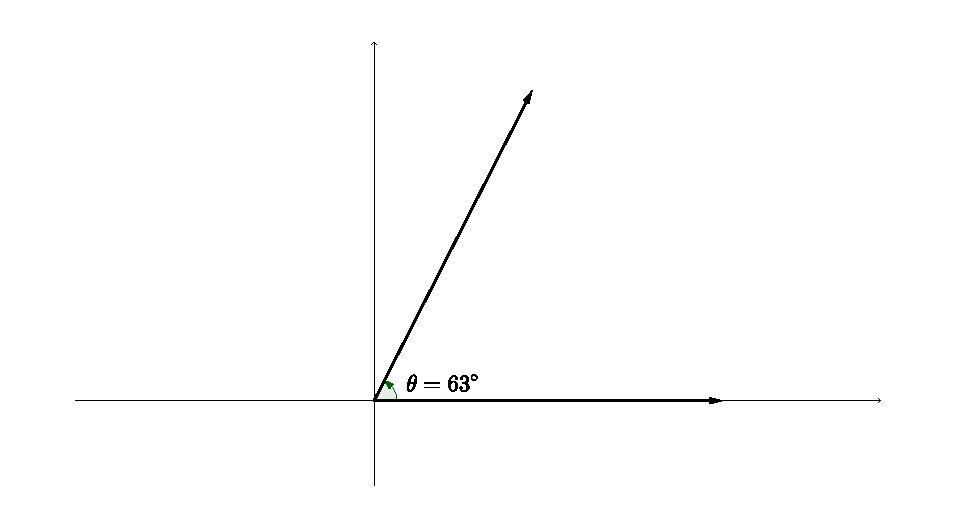
\includegraphics[scale=0.5]{63.pdf}
\end{center}}} \fi

\item $\displaystyle 400^{\circ}$

\ifans \fbox{\parbox{1\linewidth}{$\displaystyle \frac{20\pi}{9}$; 
\begin{center}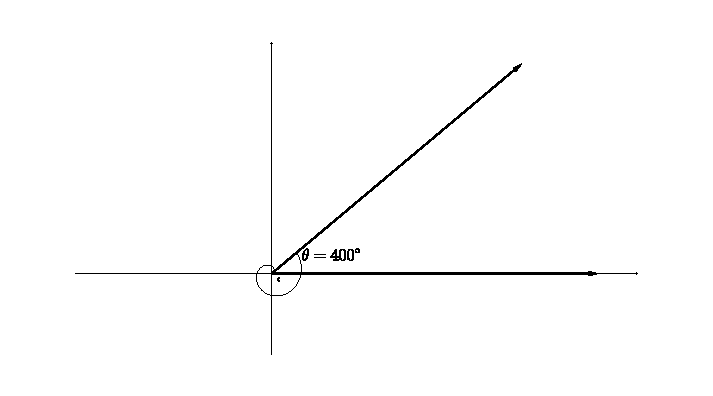
\includegraphics[scale=0.5]{400.pdf}
\end{center}}} \fi
\end{enumerate}

\item Convert the following angles from radians to degrees.  

\begin{enumerate}

\item $\displaystyle \frac{\pi}{9}$

\ifans \fbox{$\displaystyle 20^{\circ}$} \fi

\item $\displaystyle \frac{2\pi}{3}$

\ifans \fbox{$\displaystyle 120^{\circ}$} \fi

\item $\displaystyle \frac{\pi}{4}$

\ifans \fbox{$\displaystyle 45^{\circ}$} \fi

\item $\displaystyle \frac{-\pi}{6}$

\ifans \fbox{$\displaystyle -30^{\circ}$} \fi

\end{enumerate}

\item Determine the quadrant in which the terminal side of each angle lies. \newline (Each angle is measured in radians)

\begin{enumerate}

\item $\displaystyle \frac{\pi}{5}$

\ifans \fbox{Quadrant I} \fi

\item $\displaystyle \frac{11\pi}{8}$

\ifans \fbox{Quadrant III} \fi

\item $\displaystyle -\frac{\pi}{12}$

\ifans \fbox{Quadrant IV} \fi

\end{enumerate}

\item Find the length of the arc on a circle of the given radius intercepted by the given central angle.  

\begin{enumerate}

\item radius: 9 feet; central angle: $\frac{23\pi}{36}$ radians.

\ifans \fbox{$\displaystyle \frac{23\pi}{4}$ feet} \fi

\item radius: 20 centimeters; central angle: $75^{\circ}$

\ifans \fbox{$\displaystyle \frac{25\pi}{3}$ centimeters} \fi

\end{enumerate}


\item Find the area of the sector of the circle with given radius and central angle.

\begin{enumerate}

\item radius: 12 millimeters; central angle: $\displaystyle \frac{\pi}{7}$ radians

\ifans \fbox{$\displaystyle \frac{72\pi}{7}$ square millimeters} \fi

\item radius: $\displaystyle \frac{2}{3}$ inches; central angle: $63^{\circ}$

\ifans \fbox{$\displaystyle \frac{7\pi}{90}$ square inches} \fi

\end{enumerate}

\item A sprinkler system on a farm is set to spray water over a distance of 20 meters and to rotate through an angle of $140^{\circ}$.  Find the area of the region irrigated by the sprinkler.

\ifans \fbox{$\displaystyle \frac{1400\pi}{9}$ square meters}\fi


\end{enumerate}

\end{document}